\documentclass[linenumbers]{aastex631} %, twocolumn

\newcommand{\vdag}{(v)^\dagger}
\newcommand\aastex{AAS\TeX}
\newcommand\latex{La\TeX}

\usepackage{amsmath}

\begin{document}

\title{Tracking Mass Transfer between M31 and the Milky Way using Galactic Simulation Data}




\author{Avichal Kaul}
\affiliation{Steward Observatory, University of Arizona, 933 N. Cherry Ave, Tucson, AZ 85721, USA}

\keywords{Proper Motion -- local Group -- Stellar Disk --Stellar Bulge --Major Merger --Minor Merger --Dry Merger --Dynamical Friction --Jacobi Radius --Tidal Stripping/Sharing --Quenching -- Spiral Galaxy -- Tidal Tails -- Rotation Curve}

\section{Introduction}

Galactic Mergers are a process during which two or more galaxies, due to a combination of gravitational attraction and dynamic friction, fall together and merge into one galaxy. During this process, the star formation rate is increased hugely (\citep{Moster_2011}) and the structure of the galaxy undergoes massive changes - often, structures such as tidal tails are introduced, though these are not exclusive to galactic mergers. An example of one of these mergers can be seen in Figure \ref{fig:Privon image}.


Galactic mergers are an incredibly important aspect of galactic evolution. \citep{1978MNRAS.183..341W} notes that the $\lambda\text{CDM}$ model of cosmology suggests present day galaxies are formed from successive accretions and mergers of smaller entities. These successive accretions and mergers have been linked to star formation (\citep{Barnes_2004}) due to the sudden collision and compression of large HI clouds. Even the formation of tidal tails  are directly linked to the tidal forces exerted by other galaxies.explorer

A galaxy is a gravitationally bound collection of stars whose properties
cannot be explained by a combination of baryons and Newton’s laws of gravity (\citep{Willman_Strader_2012}) [where do i find a definition for galaxy evolution]

While the process of galaxies accreting and merging is well understood, there are still various open questions in this field. For instance, the role that supermassive black holes and Active Galactic Nuclei have to play during a merger. [Explain what we currently know about your chosen topic. Papers must
be cited in this paragraph. A figure must be referenced within the text to help explain
something learned about the topic (what the topic is or why it matters).]

\citep{Silverman_2011} [the role that close encounters play, and what fuels AGN activity in galaxies not undergoing mergers]. [and how we still can't explain bulge formation as a function of galactic mergers]\citep{Brooks2016}.

[What are the open questions in your chosen topic area (as defined in
Paragraph 1)? One of these open questions must relate to your specific project. How
are people trying to solve these questions? You must include citations.]

\begin{figure}
    \centering
    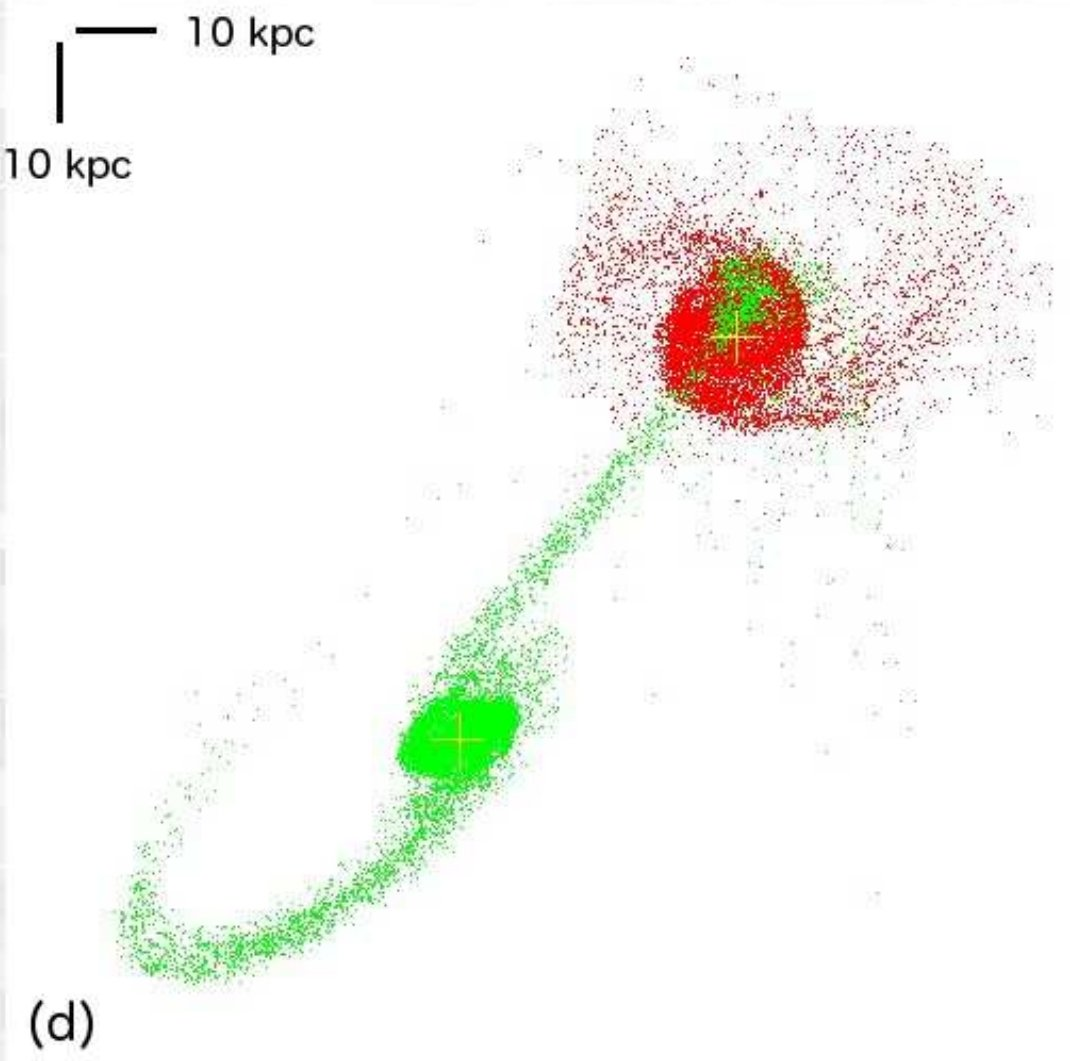
\includegraphics[width = 0.5\linewidth]{page08_1.jpg}
    \label{fig:Privon image}
    \caption{A snapshot from a galactic merger simulation that shows mass transfer between two galaxies. Figure from \citep{Privon_2013}.}
\end{figure}


\section{This Project}

In this paper, we will study the evolution of the Milky Way/M31 galactic merger. Specifically, the nature of the mass transfer during the merger and the evolution of the system with time. 

[which open question does this address?]

In the following sections, we will consider Galaxy A (stationary in its reference frame) and Galaxy B (colliding with Galaxy A). In actuality, both galaxies are moving towards each other. All the analysis described here will be performed on both the galaxies separately.

\section{Methodology}

% replace time range w/ the actual time in Gyr
Gravitational N-body simulations are numerical simulations of the equations of motion for N particles interacting gravitationally (\citep{trenti2008gravitational}). We are using N-body galactic simulations from \citep{Besla}, which provides us with a full simulation of the MW colliding with M31 over a time range of multiple Gyr. 

We wish to characterise the mass transfer at different points in the merger process. Especially of interest are the timesteps right after a close encounter, as a lot of material will be transferred between the galaxies at this time and will gradually settle into place. It will be interesting to see what material gets assimilated into another galaxy, and what material becomes gravitationally unbound. An example of what this looks like can be seen in Figure \ref{fig:Privon image}, where you can see the mass transfer between colliding galaxies. This image shows what material has been transferred, but we will also be evaluating how strongly said material is gravitationally bound. 


To check whether or not particles are gravitationally bound, we need to compare their Kinetic Energy ($T$) to their Potential Energy ($\phi$), which are given below.

\begin{gather}
T = \frac{1}{2} mv^2 \\
\phi = -\frac{GM(R)}{R}
\end{gather}

Here, $m$ is the mass of the particle, $v$ is the velocity of the particle, $G$ is the Universal Gravitational Constant,  is the mass enclosed within a radius $R$ of the galaxy. We will be using the Hernquist profile (\citep{1990ApJ...356..359H}) to find $M(R)$.

\begin{gather}
    \rho(r) = \frac{\rho}{(\frac{r}{r_s})(1+\frac{r}{r_s})^3} \\
    M(R) = [using the MassEnclosed function from HW]
\end{gather}

[add definitions for variables]

Our plots will show the location of all particles of each galaxy relative to one another projected onto a 2D representation. Some will show simple mass transfer between galaxies, while others will show which particles are gravitationally bound and which are not, and finally a representation of the velocity dispersion of particles. We can also make a 3D plot to properly discern which part of the galaxy matter has ended up in.

\subsection{Mass Transfer}

We can track the process of exchanging material by labelling the particles in the simulation with the name of their progenitor, then - after an encounter - checking to see if any particles have been exchanged between the galaxies. This only requires us to know the location of each particle, and the location of the galactic centre. For instance: we can use our previously developed code to find the location of Galaxy B's centre, and then check if any of the particles from Galaxy A have ended up there.

\subsection{Exchanged Material and its Kinematics}

To find which region of the galaxy the particles end up in, we can use a similar approach. As we know the position of the particles Galaxy A has exchanged with Galaxy B, we can check the main type of Galaxy B particle that surrounds them. Similarly, we can check if the particles rotate with the disk by calculating the velocity vector of Galaxy A's particles and comparing them to Galaxy B's particles. 

Finally, to track the total mass transfer over time, we can continue measuring how many particles have switched galaxies at regular timesteps until the galactic merger is complete.

\subsection{Evolution with Time}

I expect that, during the first couple of close encounters, most of the exchanged material will end up near the galactic centre. We can see this happening in simulation data (e.g. in Fig. \ref{fig:Privon image}). This makes sense, as the galactic centre is where most of the baryonic matter in the galaxy is concentrated. But, over time, the two galaxies will merge completely, so the material will all fall together into an elliptical galaxy.

\begin{figure}
    \centering
    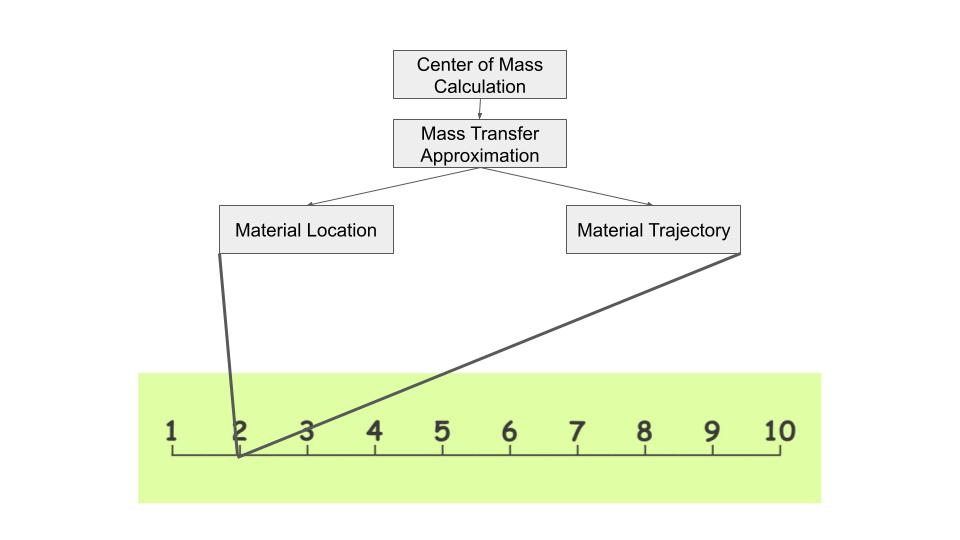
\includegraphics[width = \linewidth]{Untitled presentation.jpg}
    \label{fig:Untitled image}
    \caption{The proposed pipeline for data processing. At each simulation timestep (numbers 1-10 chosen for illustrative purposes), code is run to determine each property of the transferred material from top to bottom. This gives us an excellent idea of the evolution of the system with time.}
\end{figure}

\bibliography{sample631}{}
\bibliographystyle{aasjournal}

\end{document}
